\StartPlate{V29}{Honest phases remain a separate layer}{An action on the extension group is not yet the specified action on its representation.}
\begin{center}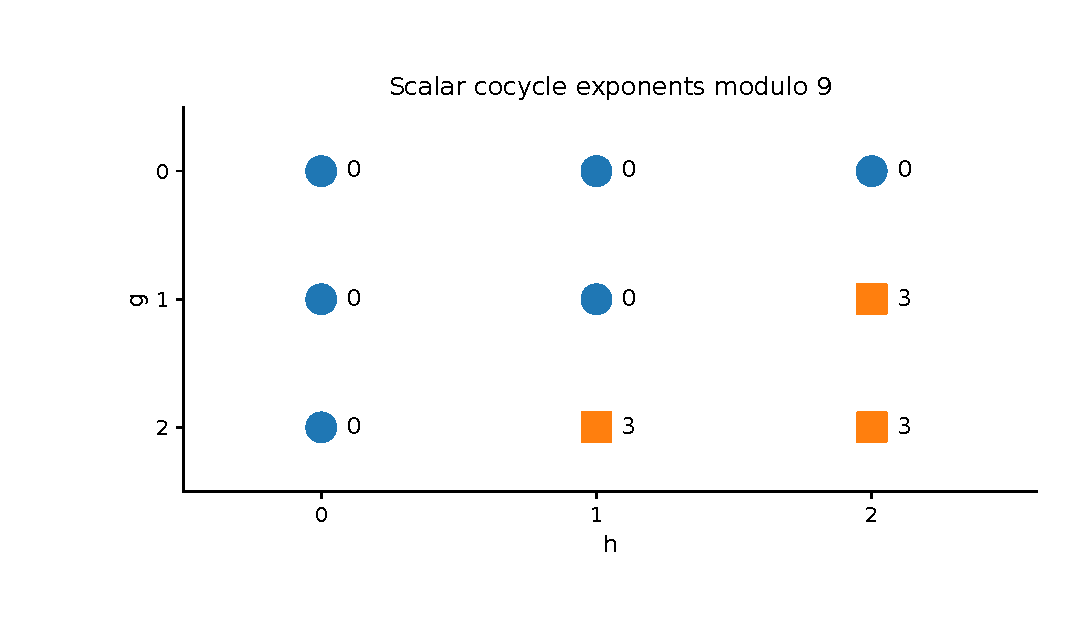
\includegraphics[width=\linewidth]{figures/V29.pdf}\end{center}
Let $g,h\in\{0,1,2\}$ represent $C_3$, and take the one-dimensional operators $U_g=\zeta_9^g$. Their multiplication has scalar discrepancy
\[
U_gU_h=\zeta_9^{c(g,h)}U_{g+h\bmod3},
\qquad c(g,h)=3\left\lfloor\frac{g+h}{3}\right\rfloor.
\]
The figure records its exponents modulo nine. Replacing $U_g$ by $\zeta_9^{-g}U_g$ gives an honest action. Yet the three honest characters $g\mapsto\zeta_3^{kg}$ are still distinct choices.

This scalar toy model isolates two separate questions: whether a projective multiplier can be removed, and which honest linearization the contract prescribes. It is not the phase system of the actual arithmetic candidate. The finite extension-action correction on V27 addresses a different discrepancy, in the group automorphisms. Canonical extension phases, Gauss conventions, and coherent transports must still be checked on the same full representation.
\vfill\PlateSource{Exact scalar projective toy model}{Part I, Section 4.2; Part III, Section 29.3}{9}
